\chapter{Aplikacja mobilna}
Aplikacja stworzona w ramach pracy pozwala na konfigurację oraz komunikację z wcześniej opisanym robotem minisumo. Z racji, iż została napisana w natywnym języku \textit{Swift} wspieranym systemem operacyjnym jest system iOS.

\section{Kompatybilność}
Jedynym wymogiem, który musi zostać spełniony w celu uruchomienia aplikacji jest wersja systemu – nie starsza niż \textit{iOS 10}. W związku z czym aplikacja z powodzeniem powinna działać zarówno na tabletach oraz telefonach marki \textit{Apple} posiadających wspomnianą lub nowszą wersję systemu. 

Docelowo aplikacja była uruchamiana oraz testowana na urządzeniu \textit{iPhone 5}, który jest najstarszym telefonem wspierającym system iOS 10. Powodem wyboru urządzenia była optymalizacja, a mianowicie poprawność działania aplikacji na najsłabszych podzespołach gwarantowała odpowiednią pracę na mocniejszych jednostkach.

Dodatkowo poprawność wyświetlania oraz skalowania została przetestowana w symulatorze dostarczonym wraz z środowiskiem \textit{Xcode} na urządzeniach takich jak \textit{iPhone 6 Plus} oraz \textit{iPad Pro}.
 
\section{Wzorzec MVC}
Aplikacja mobilna została zaprojektowana została według wzorca architektonicznego MVC (z~ang. \textit{Model–View–Controller}), który często wykorzystywany jest do tworzenia interfejsów użytkownika. W omawianym wzorcu można wyróżnić trzy obiekty:
\begin{itemize}
\item model – odpowiada za serwowanie danych,
\item widok – odpowiada za wizualizację danych, 
\item kontroler – reaguje na poczynania użytkownika, zarządza odświeżeniem widoków oraz aktualizacją modelu. 
\end{itemize}
Podział opisanych ról przedstawiono na rysunku ~\ref{fig:mvc}.
\begin{figure}[H]
	\centering
		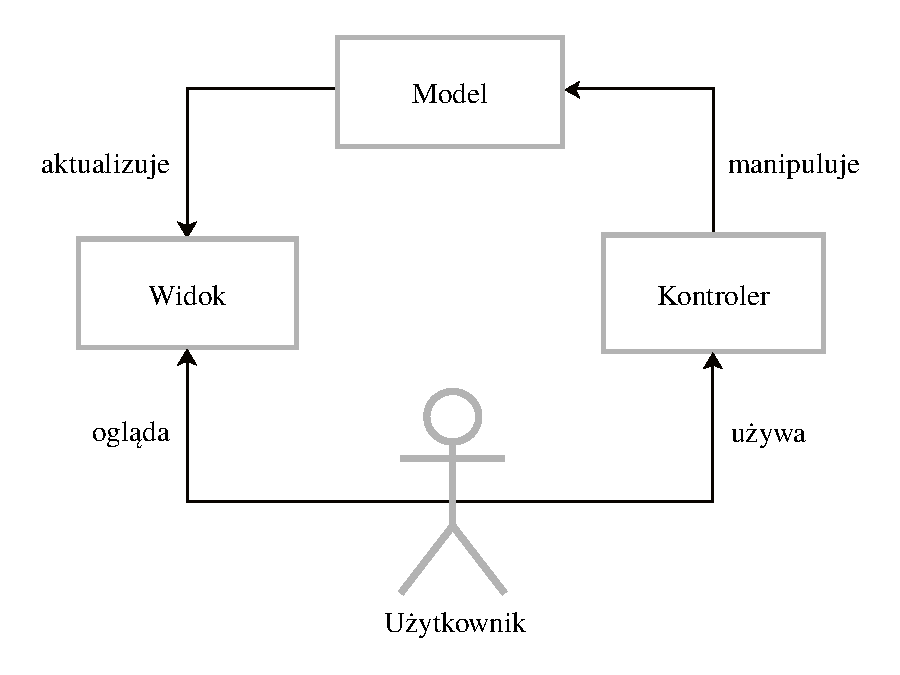
\includegraphics[width=0.75\linewidth]{pic05/mvc.pdf}
	\caption{Podział ról we wzorcu MVC.}
	\label{fig:mvc}	
\end{figure}

Dzięki wykorzystaniu tego wzorca uniezależniono przechowywane dane od sposobu w jaki są one przedstawiane użytkownikowi.

\section{Komunikacja}
Komunikacja z modułem Bluetooth została zrealizowana przy użyciu wcześniej wspomnianej platformy \textit{CoreBluetooth}. Utworzono klasę \textit{BluetoothSerial}, która była odpowiedzialna za całą logikę potrzebną do poprawnej wymiany danych między urządzeniami. Z racji, iż komunikacja jest nieodłącznym elementem każdej z funkcjonalności aplikacji skorzystano z protokołów. Protokoły są czymś na wzór intefejsów używanych w językach takich jak C++ bądź Java. Deklarują metody, lecz ich nie implementują. Każda klasa, która korzysta z komunikacji \textit{Bluetooth} musi zaimplementować metody zawarte w protokołach. Dzięki takiemu podejściu uniezależniamy logikę od kontrolerów. Klasa \textit{BluetoothSerial} nie jest w żaden sposób zależna od innych klas. Natomiast klasy, które wykorzystują komunikację, implementują odpowiednie metody w zależności od indywidualnych potrzeb.

\begin{minipage}{\textwidth}
	\begin{lstlisting}[label=protocolcode,caption=Protokół odpowiedzialny za komunikację między urządzeniami.]
protocol BluetoothSerialDelegate {
  func serialDidChangeState()
  func serialDidDisconnect(_ peripheral: CBPeripheral, error: NSError?)
  func serialDidReceiveString(_ message: String)
  func serialDidReadRSSI(_ rssi: NSNumber)
  func serialDidDiscoverPeripheral(_ peripheral: CBPeripheral, RSSI: NSNumber?)
  func serialDidConnect(_ peripheral: CBPeripheral)
  func serialDidFailToConnect(_ peripheral: CBPeripheral, error: NSError?)
  func serialIsReady(_ peripheral: CBPeripheral)
}
	\end{lstlisting}
\end{minipage}

Listing \ref{protocolcode} przedstawia zestaw metod zawartych w protokole komunikacyjnym.Poniżej przedstawiono przypadki w których zostają wywołane:

\begin{itemize}
\item \textit{serialDidChangeState} –  zmiana stanu modułu \textit{Bluetooth} (zostanie wyłączony lub włączony),
\item \textit{serialDidDisconnect} –  brak połączenia z modułem komunikacyjnym,
\item \textit{serialDidReceiveString} – została odebrana wiadomość typu tekstowego \textit{String},
\item \textit{serialDidReadRSSI} – gdy otrzymano sygnał RSSI (z ang. \textit{Received Signal Strength Indication}),
\item \textit{serialDidDiscoverPeripheral} – wykryto urządzenie podczas skanowania,
\item \textit{serialDidConnect} – połączono z urządzeniem, aczkolwiek urządzenie nie jest jeszcze gotowe na komunikację,
\item \textit{serialDidFailToConnect} – nie udało się nawiązać połączenia,
\item \textit{serialIsReady} – moduł jest gotowy na komunikację z aplikacją mobilną.
\end{itemize}

Tak jak wcześniej wspomniano, klasy korzystające z komunikacji mogą implementować dowolne z wyżej wymienionych metod w zależności od potrzeb.

\section{Struktura aplikacji}
Tak jak wcześniej wspomniano, aplikacja została stworzona przy użyciu wzorca \textit{MVC}. Poniżej przedstawiono strukturę plików aplikacji.

\begin{figure}[H]
	\centering
		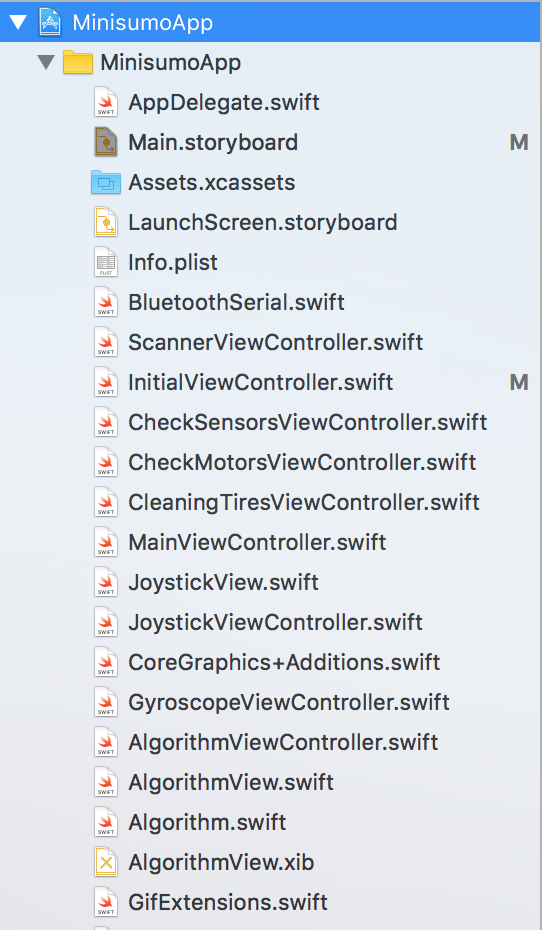
\includegraphics[width=0.75\linewidth, height=10cm, keepaspectratio]{pic05/structure.png}
	\caption{Struktura plików aplikacji mobilnej.}
	\label{fig:structure}	
\end{figure}

Na rysunku \ref{fig:structure} pliki o rozszerzeniu \textit{swift}, których nazwy kończą się na \textit{Controller} pełnią rolę kontrolerów, a \textit{View} widoków przedstawianych użytkownikowi. Reszta plików odpowiedzialna jest za logikę aplikacji. Dodatkowo plik \textit{Main.storyboard} zawiera konfiguracje większości widoków stworzonych przy użyciu graficznego narzędzia dostarczonego przez środowisko \textit{Xcode}.

\subsection{Widok główny}

\subsection{Widok sterowania automatycznego}
\subsection{Widok sterowania zdalnego}
\subsection{Widok diagnostyki}